\documentclass[onecolumn]{article}
\usepackage[utf8]{inputenc}
\usepackage[swedish,english]{babel}
\usepackage{geometry}
\usepackage{amsmath}
\usepackage{graphicx}
\usepackage{alltt}                % verbatim text with latex macros
\usepackage{xcolor}
\usepackage{tikz}
\usetikzlibrary{automata, positioning}
% instead of defining author, write your names below in Group member names
\author{}
\date{}
\title{DT2112 Lab2 Report\\Practical exercise in automatic speech recognition}

\begin{document}
\maketitle
\section*{Group member names}
\begin{itemize}
\item Sp1: Luise Dürlich (luise.durlich.9577@student.uu.se)
\item Sp2: Xiajing Li (xiajing.li.4688@student.uu.se)
\item Sp3: Chun Hung Lin (chlin3@kth.se)
\end{itemize}

\section*{Grammar explanation and graph (four digits):}
%\textcolor{teal}{I'd like to do this one (Sp1)}\\
%Copy the content of your \verb|four_digits.grm| definition and include the graph you obtained from it. What kind of utterances does this grammar allow? How was this grammar obtained by the rules you defined in \verb|four_digits.grm|?
As illustrated by the graph in figure \ref{fig:four_digits_graph}, the grammar allows utterances that consist of any four consecutive digits of the ten English denominations of digits. In figure \ref{fig:four_digits_grm}, the non-terminal \verb|$DIGIT|, is defined as any one of the ten digits. This is done by stating the digits as terminal symbols (\verb|zero| to \verb|nine|) and declaring these terminal symbols to be alternatives using the \textbar -symbol. The non-terminal \verb|$DIGIT| is then repeated four times to specify a sequence of exactly four digits within the start and end of the sentence (\verb|SENT-START| and \verb|SENT-END|) in the final command block that generates the grammar.
\begin{figure}[htbp]
  \centering
  \begin{minipage}{14cm}
    {%\small
    \begin{alltt}
$DIGIT =  zero | one | two | three | four | five | six | seven | eight | nine ;

( SENT-START $DIGIT $DIGIT $DIGIT $DIGIT SENT-END )
    \end{alltt}}
  \end{minipage}
  \caption{Contents of \texttt{four\_digits.grm}}
  \label{fig:four_digits_grm}
\end{figure}

\begin{figure}[htbp]
    \centering
    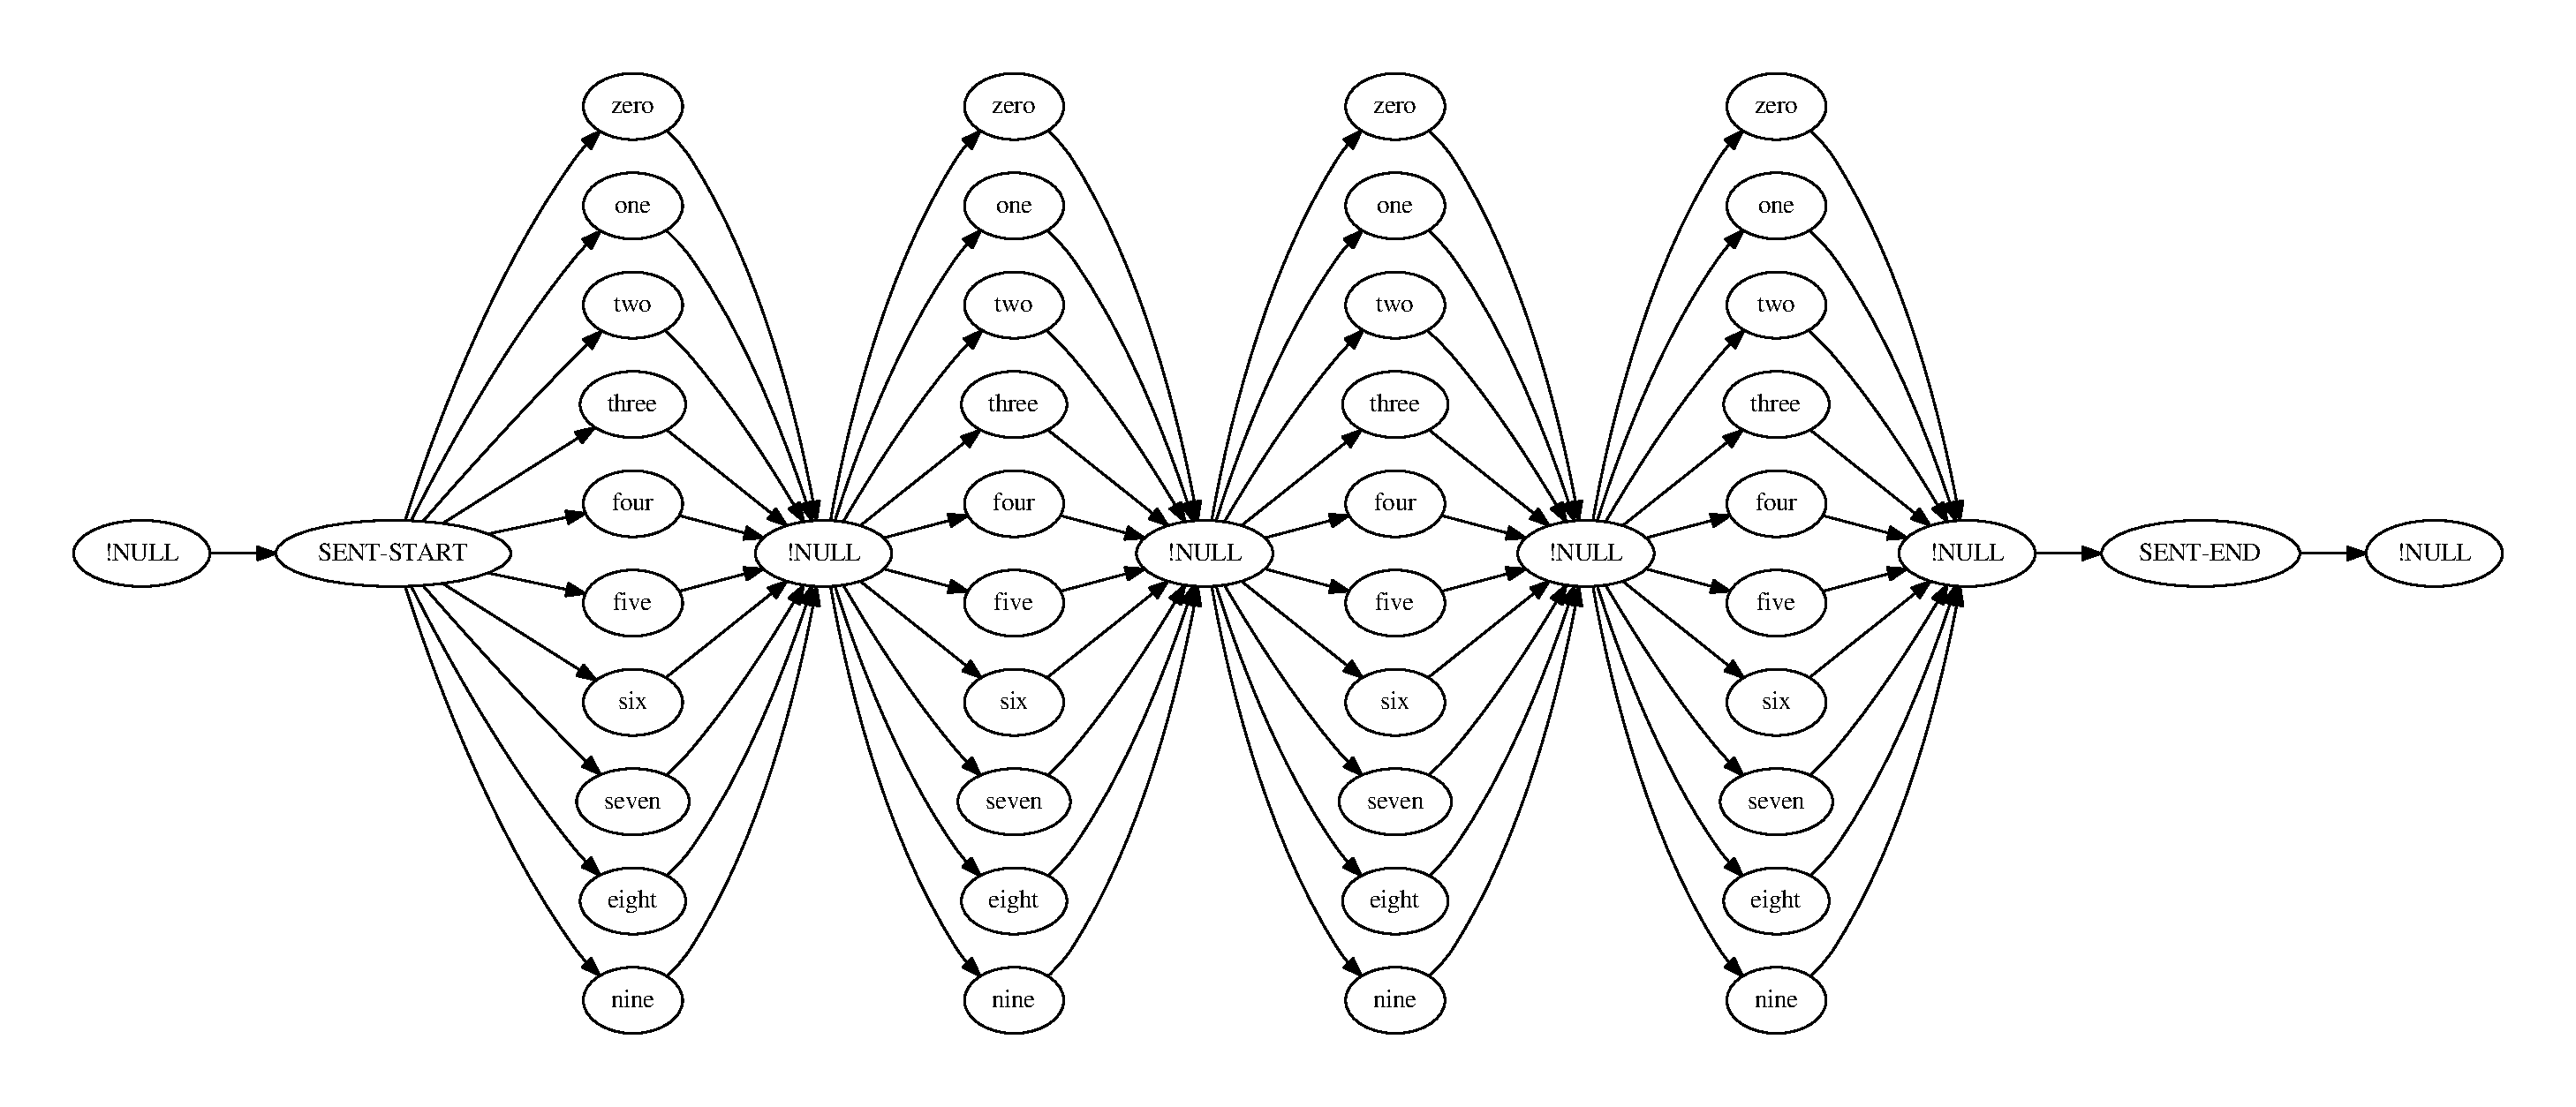
\includegraphics[height=7cm]{four_digits}
    \caption{Graph corresponding to \texttt{four\_digits.grm}}
    \label{fig:four_digits_graph}
\end{figure}

\clearpage
\section*{Grammar explanation and graph (digit loop):}
%\textcolor{teal}{I'd like to do this one (Sp1)}\\
%Copy the content of your \verb|digit_loop.grm| definition and include the graph you obtained from it. What kind of utterances does this grammar allow? How was this grammar obtained by the rules you defined in \verb|digit_loop.grm|?
The grammar defined in figure \ref{fig:digit_loop_grm} accepts any utterance composed of one or more digits. As we can see, the rule for \verb|$DIGIT| stays the same, but instead of explicitly forcing a fixed number of occurrences, it is called in a loop (\verb|<>|) in the final block. Consequently, there has to be a known digit following the start of the utterance, but after that, the utterance can either be at an end (proceeding from \verb|!NULL| directly to \verb|SENT-END|) or continue producing another digit (taking a directed edge from \verb|!NULL| to any of the digits) etc.

\begin{figure}[htbp]
  \centering
  \begin{minipage}{14cm}
    {%\small
    \begin{alltt}
$DIGIT =  zero | one | two | three | four | five | six | seven | eight | nine ;

( SENT-START <$DIGIT> SENT-END )
    \end{alltt}}
  \end{minipage}
  \caption{Contents of \texttt{digit\_loop.grm}}
  \label{fig:digit_loop_grm}
\end{figure}

\begin{figure}[htbp]
    \centering
    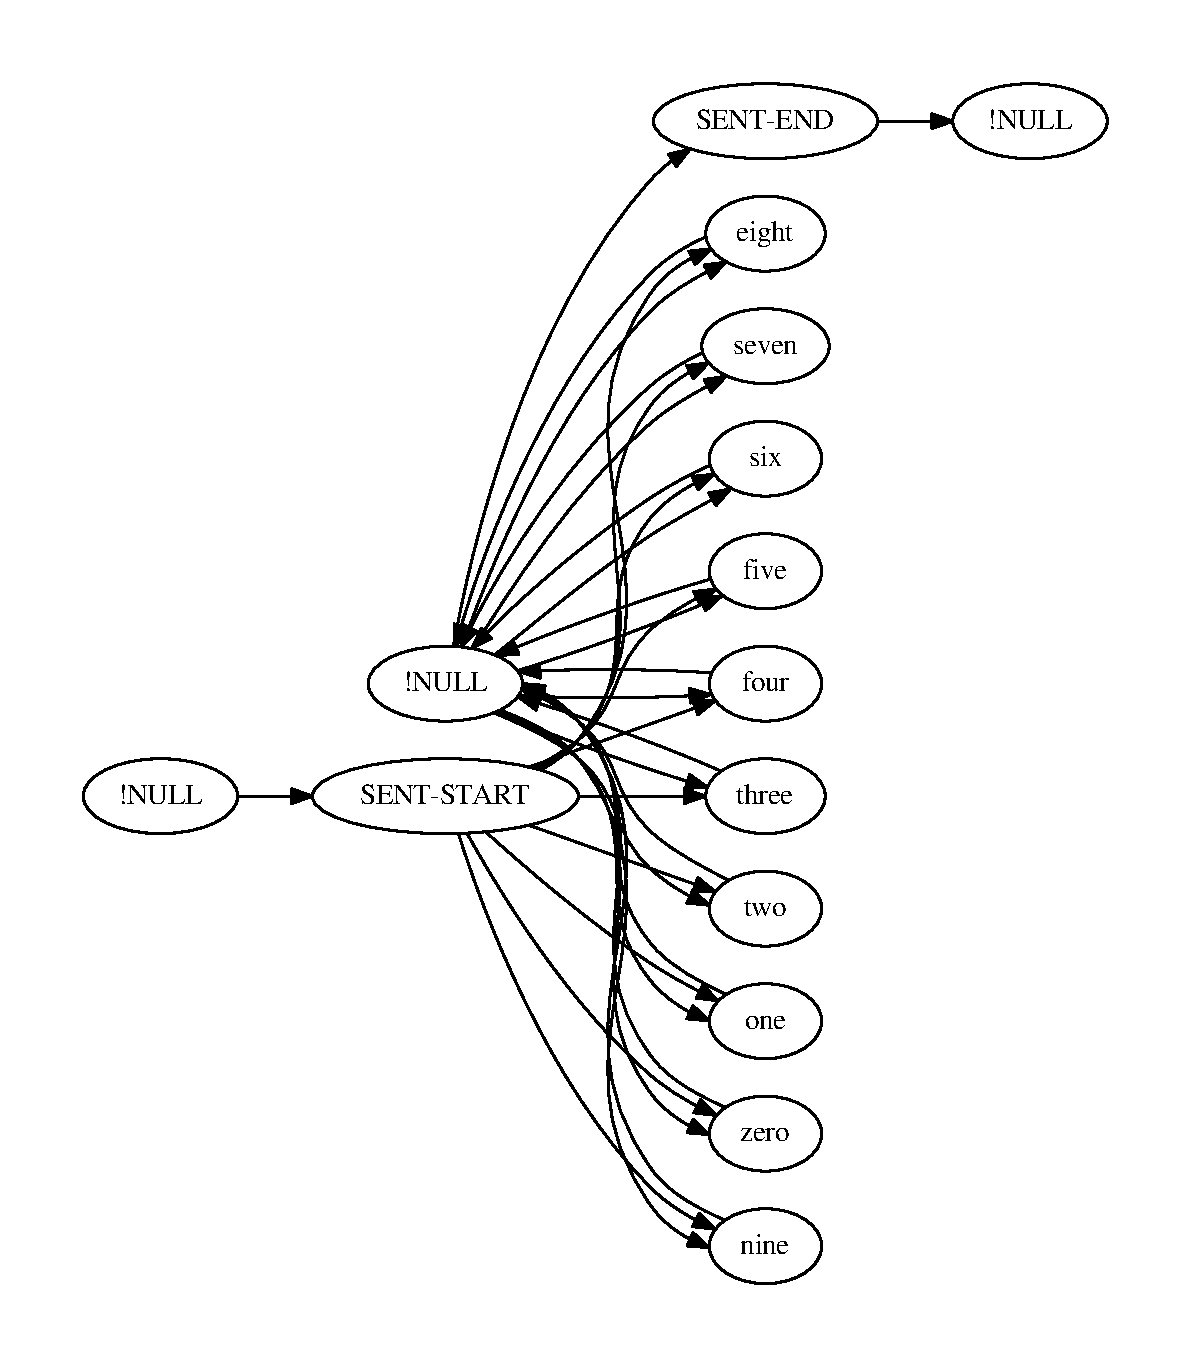
\includegraphics[height=7cm]{digit_loop}
    \caption{Graph corresponding to \texttt{digits\_loop.grm}}
    \label{fig:digit_loop_graph}
\end{figure}

\section*{Words and their phonetic transcription}
%Report the words in your dictionary and the phonetic transcriptions you have defined.
\begin{table}[htbp]
\begin{tabular}{|c|c|c|c|c|c|c|c|c|c|}
\hline
eight & five & four & nine & one & seven & six & three & two & zero \\ \hline
eI t  & f aI v  & f O:  & n A I n  & w Q n  & s e v n  & s i k s  & T r i  & t u  & z i: r ehU  \\ \hline
% cf. digits0.dic ;)
\end{tabular}
\caption{words and phonetic transcription}
\end{table}
\clearpage

\section*{Feature extraction parameters}
%These are defined in the configuration file \verb|config/features.cfg|, where times are given in 100 ns units. Convert these values into the units specified in the third column of the table. Print the contents using the command: \verb|cat config/features.cfg|.

%   The sampling frequency of the recordings is not specified in \verb|config/features.cfg|. To extract it, look at one of the files you have recorded. You can use the command \verb|file| to get information about the file, or use the file browser. In the second case right click on the file and choose the ``Properties'' option and then the ``Audio'' tab. The recordings are for each group member in the \verb|Sp$n/train_data| and \verb|Sp$n/test_data| directories\\[5mm]

%\renewcommand{\arraystretch}{1.8}
%\begin{tabular}{|l|l|p{0.3\textwidth}|}
\begin{tabular}{|l|l|l|}
\hline
Parameter & Hint & Value \\ \hline
Sampling frequency (kHz): & check recordings          & \hfill 16 (kHz) \\
Analysis window (ms):     & WINDOWSIZE (100 ns units) & \hfill 25 (ms) \\
Frame interval (ms):      & TARGETRATE (100 ns units) & \hfill 10 (ms) \\
Pre-emphasis coeff.       & PREEMCOEF                 &  0.97 \\
Filterbank \# channels    & NUMCHANS                  &  26  \\
Energy normalization      & ENORMALISE                &  False  \\
\# cepstrum coefficients  & NUMCEPS                   &  12  \\
Hamming                   & USEHAMMING                &  True  \\
\hline
\end{tabular}

\section*{Answer the following questions:}
How many speech samples are contained in one analysis window?
\\
\begin{align*}
    16 \times 1000 \times 25 \times  10^{-3} = 16 \times  25
    = 400
\end{align*}
\\
Answer: 400 samples
\\[3mm]
How much do consequent analysis windows overlap?
\\
\begin{align*}
    25 - 10 = 15 \quad \text{ms}
\end{align*}
\\
Answer: 15 ms
\\[3mm]
In a typical four digit utterance that you have recorded, how many analysis windows are used?
\\
The typical duration of four digit utterance is 3 seconds.
Therefore we have:
\begin{align*}
    (3000 - 15) \div 10 = 298.5
\end{align*}
\\
Answer: 298 analysis windows
\\[1mm]

\section*{Acoustic model parameters}
Check the prototype model definition in the file \verb|proto.mmf| and answer the following questions with the help of the HTK Book:\\
\textbf{What kind of features are used? (hint: defined in the \verb|~o| macro)}\\
\\ The features type we used is called \verb|MFCC_0_D_A|
\\[6mm]
\textbf{What is the size of the feature vector?}\\[2mm]
The size of the feature vector is 39.
This number is computed from the length of the parameterized static vector (\verb|MFCC_0| = 13) plus the delta coefficients (+13) plus the acceleration coefficients (+13).
\\[4mm]
\noindent \textbf{How many states are used per phoneme?}
\\[2mm]
We used 5 states per phoneme\\[6mm]
\textbf{Draw the topology (states and transitions) of the prototype model (Hint: \verb|TransP| is the transition probability matrix).}
\\[2mm]
The topology of the prototype model is shown in the figure \ref{fig:HMM_topo}
\\[6mm]
\begin{figure}
    \centering
    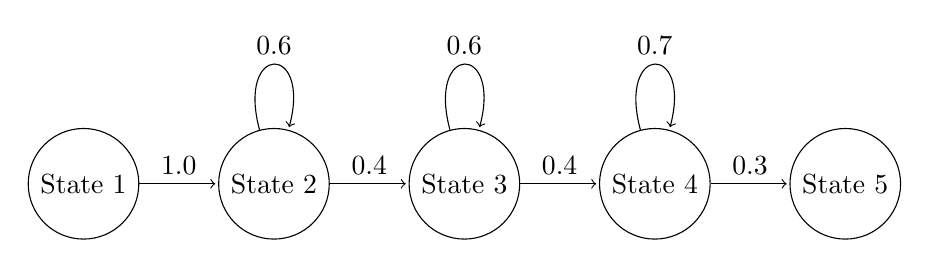
\begin{tikzpicture}
        % Add the states
        \node[state]              (s1) {State 1};
        \node[state, right=of s1] (s2) {State 2};
        \node[state, right=of s2] (s3) {State 3};
        \node[state, right=of s3] (s4) {State 4};
        \node[state, right=of s4] (s5) {State 5};

        % Connect the states with arrows
        \draw[every loop]
            (s1) edge[above=3em] node {1.0} (s2)
            (s2) edge[above=3em] node {0.4} (s3)
            (s3) edge[above=3em] node {0.4} (s4)
            (s4) edge[above=3em] node {0.3} (s5)
            (s2) edge[loop above] node {0.6} (s2)
            (s3) edge[loop above] node {0.6} (s3)
            (s4) edge[loop above] node {0.7} (s4);
    \end{tikzpicture}
    \caption{The HMM topology of the prototype model}
    \label{fig:HMM_topo}
\end{figure}

\begin{table}[ht]
\begin{tabular}{|p{0.6\textwidth}|c|p{0.15\textwidth}|}
\hline
Parameter & Hint & Value \\ \hline
Context-dependent models (yes/no) & - & No \\
Tying (yes/no)                    & - & No \\
Acoustic feature type             & \verb|<MFCC-...>| &  \verb|MFCC_0_D_A|\\
Acoustic vector size              & \verb|VecSize|    &  39  \\
\# states per phone model (incl. start and end states)  & \verb|NumStates| &  5\\
\# mixture components per state   & -    & 1 \\
\hline
\end{tabular}
\caption{The summary of acoustic model parameters}
\end{table}
\clearpage
\section*{Recognition evaluation}
Speaker dependent results: Matching the test speaker against his/her own trained models. Cross-speaker results: Matching the test speaker against another speaker’s models.\\[5mm]
%\begin{tabular}{|p{0.2\textwidth}|c|c|r|r|r|}
\begin{tabular}{|l|c|c|r|r|r|}
\hline
\textbf{4-digits}  & Training speaker(s) & Test speaker(s) & Accuracy \% & \#Ins & \#Del \\
\hline
Speaker dependent & Sp1 & Sp1 & 100 & 0 & 0 \\\hline
Speaker dependent & Sp2 & Sp2 & 97.5 & 0 &  0 \\\hline
Speaker dependent & Sp3 & Sp3 & 97.5 & 0 &  0 \\\hline
Cross-speaker & Sp1 & Sp2 & 75 & 2 & 2 \\\hline
Cross-speaker & Sp1 & Sp3 & 47.5 & 1 &  1 \\\hline
Cross-speaker & Sp2 & Sp1 & 75 & 0 & 0 \\\hline
Cross-speaker & Sp2 & Sp3 & 60 & 2 & 2 \\\hline
Cross-speaker & Sp3 & Sp1 & 72.5 & 0 & 0 \\\hline
Cross-speaker & Sp3 & Sp2 & 50 & 1 & 1 \\\hline
\end{tabular}\\[5mm]
%\begin{tabular}{|p{0.2\textwidth}|c|c|r|r|r|}
\begin{tabular}{|l|c|c|r|r|r|}
\hline
\textbf{digit-loop}  & Training speaker(s) & Test speaker(s) & Accuracy \% & \#Ins & \#Del \\
\hline
Speaker dependent & Sp1 & Sp1 & 82.5 & 7 & 0 \\\hline
Speaker dependent & Sp2 & Sp2 & 97.5 & 0 & 0 \\\hline
Speaker dependent & Sp3 & Sp3 & 95 & 1 & 1 \\\hline
Cross-speaker & Sp1 & Sp2 & 47.5 & 13 & 0 \\\hline
Cross-speaker & Sp1 & Sp3 & 10 & 15 & 0 \\\hline
Cross-speaker & Sp2 & Sp1 & 70 & 2 & 2 \\\hline
Cross-speaker & Sp2 & Sp3 & 60 & 3 & 1 \\\hline
Cross-speaker & Sp3 & Sp1 & 47.5 & 10 & 0 \\\hline
Cross-speaker & Sp3 & Sp2 & 27.5 & 11 & 1 \\\hline
\end{tabular}


\clearpage
\section*{Discussion of the results}
\textbf{Common digit confusions:}\\
We notice several groups of common digits confusions: 
\textbf{(1)} \texttt{three}, \texttt{seven} and \texttt{six}, \textbf{(2)} \texttt{one}, \texttt{eight} and \texttt{nine} and \textbf{(3)} \texttt{two} and \texttt{three}, as well as a high number of insertions of \texttt{six}.

\vspace{0.3cm}

\noindent \textbf{These might have been caused by:}\\
The occurrence of the same or similar consonants and vowels: \texttt{seven} and \texttt{six} for example resemble each other in the beginning, as they both start with an \texttt{s} and vowels that do not differ too much in terms of the formants that can be observed (cf. the second and third wave and the corresponding spectogram in figure \ref{fig:record1}) . Similarly, \texttt{two} and \texttt{three} start on relatively similar consonants -- at least as far as the place of articulation is concerned and in cases where the \texttt{t} is not overly aspirated -- and the vowels make for two soundwave representation that seem to be quite alike.
\begin{figure}[htbp]
    \centering
    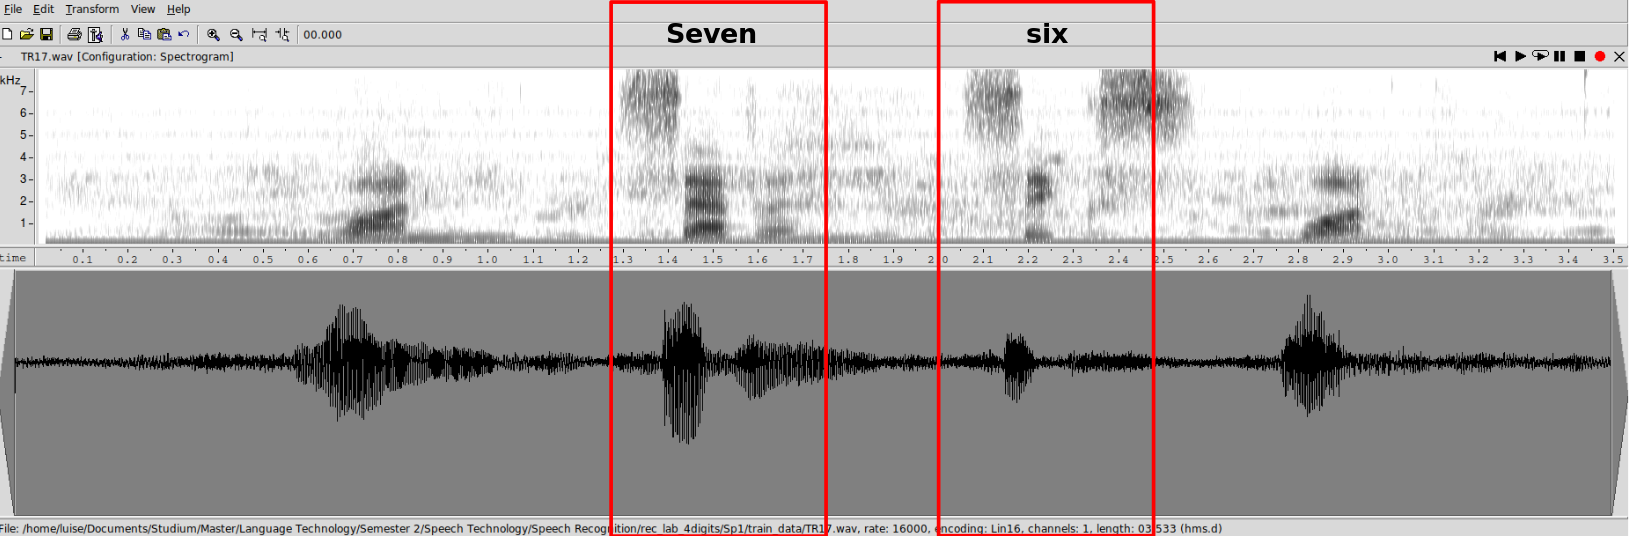
\includegraphics[width=15cm]{one_seven_six_one}
    \caption{Spectrum of record 'one seven six one'}
    \label{fig:record1}
\end{figure}
\\
Upon reviewing the recordings for \texttt{eight} and \texttt{nine}, we observed that in some cases the final consonant had not been pronounced or was inaudible in given the volume of the different speakers and the environment. This lead to confusion when training and applying the model.\\
\\
The insertion of \texttt{six} is most likely due to some soft-voiced recordings in which the digit fades into the background.\\
\\
\noindent \textbf{Compare and discuss the difference between the cross-speaker and the speaker-dependent results.}\\
In speaker-dependent evaluation, it is reasonable to get higher accuracy results of recognition, because generally, the voice features of one particular person remain stable. Only few errors occur and might be due to the speaking rate on speaker. However, in cross-speaker evaluation, since pronunciation and features of voice vary from person to person,the accuracy decrease almost by half. For two of the speakers, Sp1 and Sp2, who are both female, we can observe higher cross-speaker accuracy than compared to cross-speaker results with Sp3, which is most likely due to more similar recordings in terms of pitch.\\
\\
\noindent \textbf{How do the performance and types of errors differ between recognition of fixed and non-restricted number of digits (digit loop)?}\\
There are three types of errors showed in the HTK Results Analysis: I=insertions, S=substitutions, D=deletions. Speaker-dependent evaluation shows that the performance is similar between recognition of fixed and non-restricted number of digits. However, experiments based on \emph{Sp1} and \emph{Sp3} with digits loop get almost half of the accuracy of fixed number recognition. These results show less influence on deletion while errors mainly come from the high insertion of unnecessary words. It might because there is no limitation of numbers of digits to be recognized so that sometimes recognizer would take background noise into consideration. 

\section*{Experience with the live recogniser}
\noindent \textbf{How does the recogniser behave when you use it live?}
\\[1mm]
Using live recogniser in \emph{Wavesurfer} is very convenient to see the immediate recognition result when changing some parameters. With the same speaker as during training, the majority of digits uttered is recognised correctly. However, in some models, % was it Sp1 and Sp3 or all the models? and did we have problems recognising certain digits for the same speaker? Yes.
there are insertions between the actual digits.\\
\\
\noindent \textbf{What is the effect of varying the speaking rate?}\\
For a low speaking rate, the recogniser can recongnise digits correctly. 
We tested two sequences of digits: "one seven one six" and "nine one two three". \\
\\
For a high speaking rate, there were two situations. 
In recording our sounds for training and testing, typically we spent 3 or 4 seconds.
When we said 4 digits in 2.5 seconds, it still able to recongnise part of the digits.
When we said 4 digits in 1 seconds, it can not recongnise any digits.\\
\\
We tested another two sequences of digits: "nine nine one one" and "one six zero one".
\\
%\noindent what is the effect of varying the insertion penalty?\\
\\
\textbf{What is the effect of varying the insertion penalty?}
Insertion penalty can change the the transition from the end of one word to the start of the next. Larger negative insertion penalty can result in more deletion errors and less insertion errors, while larger positive insertion penalty can result in more insertion errors and less deletion errors. During the experiment the most common word insertion is the word \texttt{three}. A higher insertion penalty on the other hand leads to a lot more insertions between actual uttered words.\\
\\

\noindent \textbf{How does the recogniser cope with long pauses between words? Can you change the behaviour using the insertion penalty?}%\textheight}
The recogniser deals with long pauses in different ways depending on the model and speaker. For the model trained on Sp1 data for example, longer pauses between two digits are almost always interpreted as the digit \texttt{three}. By lowering insertion penalty to $-100$, this overgeneration of digits can be curtailed to some extent.\\ %if I remember correctly%

\noindent \textbf{What happens when you include an optional silence ``word'' between each digits in the grammar?}\\
The introduction of a silence word(SIL [] sil) improves the performance such that long pauses are no longer interpreted as digits. By doing so the system takes pause into consideration into consideration automatically so that the insertion would be reduced.\\

\noindent \textbf{What words did you add to the dictionary and grammar? How did the recogniser perform with them?}\\
As new words with phonemes that are already recorded in the test data, we added \texttt{fine} (\texttt{f~aI~n}) and \texttt{no} (\texttt{n~O:}) to the dictionary. We found that the recogniser did a good job at identifying these words even though it did not encounter them in the soundfiles during training. It would have been interesting to see how the recogniser performs on longer words, but unfortunately it was quite hard to come up with examples based on the phonemes already in the dictionary.\\
\\

\noindent \textbf{Using the live recogniser, try recording while holding the microphone a different distances from your mouth. Can you see any difference in the recognition accuracy?}\\
When the microphone was about 4 cm from our tester's mouth, the recognition accuracy was still high. It can recognize all digits correctly.\\
\\
When the microphone was close to tester's mouth, It received extra noise and made some extra digits, but for the signal we want to recognize it still gave correct results.
\end{document}
